\documentclass[11pt,twocolumn,letterpaper]{article}

\usepackage{cvpr}
\usepackage{times}
\usepackage{epsfig}
\usepackage{graphicx}
\usepackage{amsmath}
\usepackage{amssymb}
\usepackage{pifont}
\newcommand{\cmark}{\ding{51}}%

\usepackage[utf8]{inputenc}
\usepackage[T1]{fontenc}

\usepackage[breaklinks=true,bookmarks=false]{hyperref}
\usepackage{enumitem}

\cvprfinalcopy % *** Uncomment this line for the final submission

\def\cvprPaperID{****} % *** Enter the CVPR Paper ID here
\def\httilde{\mbox{\tt\raisebox{-.5ex}{\symbol{126}}}}

\begin{document}

%%%%%%%%% TITLE
\title{Challenge Data ``POSOS: Predict the expected answer"}

\author{Romain Vial\\ \texttt{romain.vial@mines-paristech.fr}}

\maketitle

\section{Introduction}

In France, more than 11,000 drugs are currently commercialized. Not only patients but also healthcare professionals are struggling with their usage. More importantly, drug misuse could be responsible for more than 144,000 hospitalizations every year in France, and more than 1.5 million in the USA.

What is particularly interesting to understand about drug queries is what information people actually expect as an answer. This could be for instance side effects, drug composition or contraindication. While there is a limited number of question types, the challenge lies in the diversity and variability of the questions asked.

The goal of the POSOS challenge is to predict the intent associated to a given question. Questions are classified according to a list of 51 different anonymized categories. To solve this problem, we explored different classical text classification methods and combined them to provide an acceptable answer.

In the following sections, we will first focus on understanding the data. Then, we will describe the proposed algorithm. Finally, we will present our results and ranking.

\section{Data Exploration}

First, we will try to explore and understand the data before doing any further processing.

The dataset is made of 10,063 questions, where 8028 questions and their corresponding intents are used for training, and 2035 questions without any intent used for testing. 

\subsection{Class Imbalance}

The questions are distributed among 51 anonymized intents or categories. Figure~\ref{fig:intent_hist} shows the intent distribution over the training set. One can see that the dataset is badly imbalanced. The class \texttt{28} accounts for more than 22\% of the dataset while around 30 classes account for less than 1\% each. We can assume that the test set has the same distribution. However, dealing with imbalanced distribution can harm our future classification results.

\begin{figure}
\centering
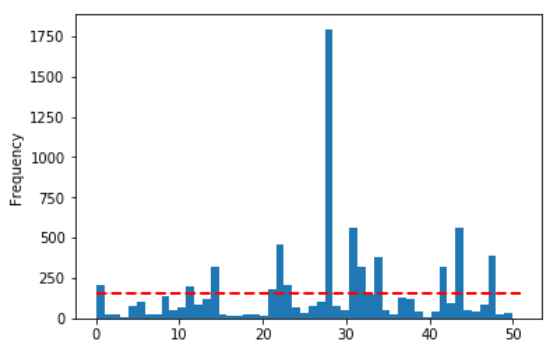
\includegraphics[width=0.9\linewidth]{images/intent_hist}
\caption{Intent distribution over the training set. In red, the corresponding uniform distribution. Best viewed in colors.}
\label{fig:intent_hist}
\end{figure}

\subsection{Dealing with Drug Names}
\label{sec:drug-names}

Most of the questions in the dataset contain several drug names. Our assumption is that for this intent classification task, the presence and count of drug names is actually more important than the actual names. For instance, in the sentence ``Par quoi remplacer Aerius pendant la grossesse ?", the name ``Aerius" is not that important for classification as long as we can recognize that the sentence contains one drug name. We could even replace the drug name by a token, ``Par quoi remplacer <MED> pendant la grossesse ?", without losing too much information.

In this project, we used three strategies to deal with these drug names:
\begin{enumerate}
\item adding a numerical features containing the number of occurrences of any drug names in the question
\item replacing all occurrences of drug names by a token <MED>
\item replacing all occurrences of drug names by a numbered token, e.g. if two drugs appear in the question, one will be replaced by <MED0> and the other one by <MED1>
\end{enumerate}

The extraction of drug names in a given question is done by looking for any occurrence of a known drug commercialized in France. The list of drug commercialized in France is openly available on the ANSM website\footnote{ANSM website: \texttt{www.agence-prd.ansm.sante.fr}}.

\section{Proposed Approach}

In the following section, we will present the methods used to represent and classify the questions. 

\subsection{Feature Representation}

% Meaningful features

\subsubsection{TF-IDF}

A common representation for textual data is the so-called Bag-of-Words (BoW) representation where each sentence is represented as an histogram of term occurrence. Hence, each individual token is treated as a feature. However, in a large text corpus some words will be over-represented, such as ``the" or ``a" in English, thus carrying little information about the actual category of the sentence. Furthermore, these words will disturb the statistics of rarer but discriminative words.

Tf-idf, term frequency times inverse document frequency, is a reweighing scheme aiming at reflecting how important is a word to a sentence or document. The simplest choice for the term frequency is to use the raw count of a term in a document, i.e. the BoW frequency. Then, the inverse document frequency is a measure of how much information this word carries. Basically, a word that is rare in the whole corpus will probably provide more information than a very common word. A simple choice for the idf term is the opposite logarithm of the number of documents containing this term divided by the total number of documents. This leads to the following formula:
\begin{align*}
\text{tf-idf}(t,d) &= \text{tf}(t, d) \times \text{idf}(t)\\
&= f_{t,d} \times \log\left(\frac{N}{n_{t}}\right)
\end{align*}
where $f_{t,d}$ is the frequency of term $t$ in document $d$, $N$ is the total number of documents and $n_{t}$ is the number of documents containing the term $t$.

\subsubsection{Doc2Vec}

Doc2Vec \cite{le2014distributed} is a distributed representation of documents, built as an extension of the more classical Word2Vec \cite{mikolov2013distributed}. Its idea is to embed document into a high-dimensional space where similar documents tend to be close to each other. Contrary to the tf-idf approach, the distance between two document vectors carries a meaning.

The document vectors are obtained after an unsupervised training phase where the model tries to predict the next word in a sentence given its context and a document vector. Such representation has been proven useful in sentiment analysis or other classification tasks.

\subsection{Classification Method}

\subsubsection{Support Vector Machine}

Support Vector Machine (SVM) is a classical method to perform supervised classification. It was first proposed and described by \cite{Cortes1995}. The idea is to embed the input data into a high-dimensional space where the data become linearly separable. In our case, as our data already live in a high-dimensional space, we only used a simple linear kernel.

\subsubsection{Xgboost}

Xgboost \cite{chen2016xgboost} is a boosting method based on an ensemble of classification trees. Contrary to SVM, the model is here trained in an additive manner. Basically, this means that at each iteration of the training process, it tries to find the tree that most improves the model according to some loss function and regularization score.

\subsubsection{Ensembling}

The idea to combine the output of different classifiers into a new one to boost predictive performance is called ensembling. In practice, an ensemble model yield better results when there is a significant diversity among models.

\section{Experiments}

In order to assess the interest of our method, we performed several quantitative and qualitative experiments. In the following, the training set is separated into two splits: 80\% for training and 20\% for validating. 

\subsection{Quantitative Experiments}

Table~\ref{tab:experiments} shows the training and validation accuracy according to different representation and classification models. When two classification models are checked, it means that we use an ensemble of the two model. We use a simple ensemble strategy which consists at outputting a weighted average of both SVM and Xgboost probabilities.

One can see that the Doc2Vec approach results in a much lower accuracy than the tf-idf approach. Some insights about this result can be found in Sec.~\ref{sec:qualitative-exp}. The tf-idf approach looks more robust in this classification task. We can also observe that, in both cases, ensembling the results of SVM and Xgboost leads to a slight improvement of the accuracy.

According to these results, we chose to submit our tf-idf ensembling approach in order to evaluate it on the test set. We have been able to obtain an accuracy of 68.60\%, which is the 8th position (out of 19) including the POSOS benchmark.

\begin{table}[t!]
\centering
\begin{tabular}{|c|c||c|c||c|c|}
\hline
tf-idf & Doc2Vec & SVM & XGB & train & val\\
\hline
\hline
\cmark & & \cmark & & 99.41 & 65.91 \\
\hline
\cmark & & & \cmark & 94.11 & 60.50 \\
\hline
\cmark & & \cmark & \cmark & 99.37 & \textbf{66.71} \\
\hline
\hline
& \cmark & \cmark & & 84.28 & 51.84 \\
\hline
& \cmark & & \cmark & 98.65 & 50.18 \\
\hline
& \cmark & \cmark & \cmark & 93.98 & 52.03 \\
\hline
\end{tabular}
\caption{Train and val accuracy according to different representation and classification models.}
\label{tab:experiments}
\end{table}

\subsection{Qualitative Experiments}
\label{sec:qualitative-exp}

One interest of using Doc2Vec as a distributed representation for our data, is to be able to plot and explore the embedding space. Figure~\ref{fig:embedding} shows the Doc2Vec embedding of the training split. One can see that classes are not well separated. This actually explains the poor results obtained with this method compared with the classical tf-idf approach.

\begin{figure}
\centering
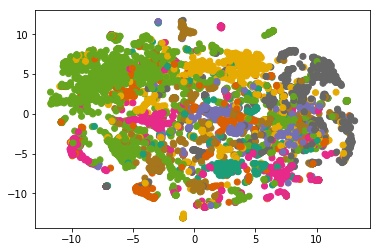
\includegraphics[width=0.95\linewidth]{images/embedding}
\caption{T-SNE representation of the 50-dimensional Doc2Vec embedding of the training split. The color of a point represents the intent of the corresponding question. Best viewed in colors.}
\label{fig:embedding}
\end{figure}

\section{Conclusion}

% Normalization, Med embedding, CNN/RNN

In this report, we tried several data representations along with supervised classifiers to recognize intent in medical questions. We haven't been able to reach Posos's state-of-the-art at 84.69\%, thus obtained a reasonable result around 69\% without using advanced methods such as Convolutional Neural Networks. In the following, we will describe some of the possible improvements to our method that could boost the results:
\begin{itemize}
\item We actually observed that many sentences contain spelling errors or unnormalized French, such as punctuation repetitions or phonetic spelling. Such words are usually harmful as they will be counted as out of the vocabulary tokens. This could be one possible reason for the poor results of the Doc2Vec approach. Such normalization method could be implemented following noisy channel based spelling correction approaches as proposed by \cite{kernighan1990spelling}. 

\item The way we treated drug names is actually very simple by either replacing names by a common token or adding a new feature containing the number of occurrences (cf. Sec.~\ref{sec:drug-names}). Another possible method would have been training drug embeddings. For instance, by looking at which drugs co-occur in the same question or context, we could have probably extracted interesting insights to improve the overall representation of a question. 

\item Convolutional and Recurrent Neural Networks have recently proven their superior capabilities to capture semantic and syntactic features in natural language. Combining them with well trained word vectors, possibly specialized on a medical corpus, would probably boost our classification accuracy.
\end{itemize}


{\small
\bibliographystyle{ieee}
\bibliography{egbib}
}

\end{document}